% Options for packages loaded elsewhere
\PassOptionsToPackage{unicode}{hyperref}
\PassOptionsToPackage{hyphens}{url}
%
\documentclass[
  english,
  man]{apa6}
\usepackage{lmodern}
\usepackage{amssymb,amsmath}
\usepackage{ifxetex,ifluatex}
\ifnum 0\ifxetex 1\fi\ifluatex 1\fi=0 % if pdftex
  \usepackage[T1]{fontenc}
  \usepackage[utf8]{inputenc}
  \usepackage{textcomp} % provide euro and other symbols
\else % if luatex or xetex
  \usepackage{unicode-math}
  \defaultfontfeatures{Scale=MatchLowercase}
  \defaultfontfeatures[\rmfamily]{Ligatures=TeX,Scale=1}
\fi
% Use upquote if available, for straight quotes in verbatim environments
\IfFileExists{upquote.sty}{\usepackage{upquote}}{}
\IfFileExists{microtype.sty}{% use microtype if available
  \usepackage[]{microtype}
  \UseMicrotypeSet[protrusion]{basicmath} % disable protrusion for tt fonts
}{}
\makeatletter
\@ifundefined{KOMAClassName}{% if non-KOMA class
  \IfFileExists{parskip.sty}{%
    \usepackage{parskip}
  }{% else
    \setlength{\parindent}{0pt}
    \setlength{\parskip}{6pt plus 2pt minus 1pt}}
}{% if KOMA class
  \KOMAoptions{parskip=half}}
\makeatother
\usepackage{xcolor}
\IfFileExists{xurl.sty}{\usepackage{xurl}}{} % add URL line breaks if available
\IfFileExists{bookmark.sty}{\usepackage{bookmark}}{\usepackage{hyperref}}
\hypersetup{
  pdftitle={The title},
  pdfauthor={Makayla Whitney1, Ernst-August Doelle1, Ernst-August Doelle1, \& Ernst-August Doelle1},
  pdflang={en-EN},
  pdfkeywords={keywords},
  hidelinks,
  pdfcreator={LaTeX via pandoc}}
\urlstyle{same} % disable monospaced font for URLs
\usepackage{graphicx,grffile}
\makeatletter
\def\maxwidth{\ifdim\Gin@nat@width>\linewidth\linewidth\else\Gin@nat@width\fi}
\def\maxheight{\ifdim\Gin@nat@height>\textheight\textheight\else\Gin@nat@height\fi}
\makeatother
% Scale images if necessary, so that they will not overflow the page
% margins by default, and it is still possible to overwrite the defaults
% using explicit options in \includegraphics[width, height, ...]{}
\setkeys{Gin}{width=\maxwidth,height=\maxheight,keepaspectratio}
% Set default figure placement to htbp
\makeatletter
\def\fps@figure{htbp}
\makeatother
\setlength{\emergencystretch}{3em} % prevent overfull lines
\providecommand{\tightlist}{%
  \setlength{\itemsep}{0pt}\setlength{\parskip}{0pt}}
\setcounter{secnumdepth}{-\maxdimen} % remove section numbering
% Make \paragraph and \subparagraph free-standing
\ifx\paragraph\undefined\else
  \let\oldparagraph\paragraph
  \renewcommand{\paragraph}[1]{\oldparagraph{#1}\mbox{}}
\fi
\ifx\subparagraph\undefined\else
  \let\oldsubparagraph\subparagraph
  \renewcommand{\subparagraph}[1]{\oldsubparagraph{#1}\mbox{}}
\fi
% Manuscript styling
\usepackage{upgreek}
\captionsetup{font=singlespacing,justification=justified}

% Table formatting
\usepackage{longtable}
\usepackage{lscape}
% \usepackage[counterclockwise]{rotating}   % Landscape page setup for large tables
\usepackage{multirow}		% Table styling
\usepackage{tabularx}		% Control Column width
\usepackage[flushleft]{threeparttable}	% Allows for three part tables with a specified notes section
\usepackage{threeparttablex}            % Lets threeparttable work with longtable

% Create new environments so endfloat can handle them
% \newenvironment{ltable}
%   {\begin{landscape}\begin{center}\begin{threeparttable}}
%   {\end{threeparttable}\end{center}\end{landscape}}
\newenvironment{lltable}{\begin{landscape}\begin{center}\begin{ThreePartTable}}{\end{ThreePartTable}\end{center}\end{landscape}}

% Enables adjusting longtable caption width to table width
% Solution found at http://golatex.de/longtable-mit-caption-so-breit-wie-die-tabelle-t15767.html
\makeatletter
\newcommand\LastLTentrywidth{1em}
\newlength\longtablewidth
\setlength{\longtablewidth}{1in}
\newcommand{\getlongtablewidth}{\begingroup \ifcsname LT@\roman{LT@tables}\endcsname \global\longtablewidth=0pt \renewcommand{\LT@entry}[2]{\global\advance\longtablewidth by ##2\relax\gdef\LastLTentrywidth{##2}}\@nameuse{LT@\roman{LT@tables}} \fi \endgroup}

% \setlength{\parindent}{0.5in}
% \setlength{\parskip}{0pt plus 0pt minus 0pt}

% \usepackage{etoolbox}
\makeatletter
\patchcmd{\HyOrg@maketitle}
  {\section{\normalfont\normalsize\abstractname}}
  {\section*{\normalfont\normalsize\abstractname}}
  {}{\typeout{Failed to patch abstract.}}
\patchcmd{\HyOrg@maketitle}
  {\section{\protect\normalfont{\@title}}}
  {\section*{\protect\normalfont{\@title}}}
  {}{\typeout{Failed to patch title.}}
\makeatother
\shorttitle{Title}
\keywords{keywords\newline\indent Word count: X}
\DeclareDelayedFloatFlavor{ThreePartTable}{table}
\DeclareDelayedFloatFlavor{lltable}{table}
\DeclareDelayedFloatFlavor*{longtable}{table}
\makeatletter
\renewcommand{\efloat@iwrite}[1]{\immediate\expandafter\protected@write\csname efloat@post#1\endcsname{}}
\makeatother
\usepackage{csquotes}
\ifxetex
  % Load polyglossia as late as possible: uses bidi with RTL langages (e.g. Hebrew, Arabic)
  \usepackage{polyglossia}
  \setmainlanguage[]{english}
\else
  \usepackage[shorthands=off,main=english]{babel}
\fi

\title{The title}
\author{Makayla Whitney\textsuperscript{1}, Ernst-August Doelle\textsuperscript{1}, Ernst-August Doelle\textsuperscript{1}, \& Ernst-August Doelle\textsuperscript{1}}
\date{}


\authornote{

Add complete departmental affiliations for each author here. Each new line herein must be indented, like this line.

Enter author note here.

The authors made the following contributions. Makayla Whitney: Conceptualization, Writing - Original Draft Preparation, Writing - Review \& Editing; Ernst-August Doelle: Writing - Review \& Editing; Ernst-August Doelle: Writing - Review \& Editing; Ernst-August Doelle: Writing - Review \& Editing.

Correspondence concerning this article should be addressed to Makayla Whitney, Postal address. E-mail: \href{mailto:my@email.com}{\nolinkurl{my@email.com}}

}

\affiliation{\vspace{0.5cm}\textsuperscript{1} University of Oregon}

\abstract{
One or two sentences providing a \textbf{basic introduction} to the field, comprehensible to a scientist in any discipline.

Two to three sentences of \textbf{more detailed background}, comprehensible to scientists in related disciplines.

One sentence clearly stating the \textbf{general problem} being addressed by this particular study.

One sentence summarizing the main result (with the words ``\textbf{here we show}'' or their equivalent).

Two or three sentences explaining what the \textbf{main result} reveals in direct comparison to what was thought to be the case previously, or how the main result adds to previous knowledge.

One or two sentences to put the results into a more \textbf{general context}.

Two or three sentences to provide a \textbf{broader perspective}, readily comprehensible to a scientist in any discipline.
}



\begin{document}
\maketitle

\hypertarget{introduction}{%
\section{Introduction}\label{introduction}}

Our project was built around two datasets detailing head counts of students with exceptionalities eligible for special education services aged 6-21. The datasets detail the categorization for special education eligibility in public schools within British Columbia and Oregon. The head counts from BC are collected from 1996/1997 to the most recent data from 2019/2020. The OR head counts include years 2002-2020. Levels of categorization include school- district- and provincial-level head counts for BC. The OR data set includes state-wide head counts that are not aggregated by school or district.

We intend to explore several questions regarding longitudinal trends. Firstly, we hope to analyze trends in disability prevalence over time. We will engage in a discussion on developmental trajectories by studying how trends shift from static/linear to increasing linear trends based on age of diagnosis for the Oregon data, which can serve as a springboard to make inferences about BC data. In studying the differences and similarities between the two datasets we will also engage in a discussion on diagnosis terminology across regions with respect to the definitions as detailed by the Diagnostic and Statistical Manual of Mental Disorders (DSM), in part as a response to a challenge set by differing terminology between BC/OR categorization.

Secondly, we hope to more closely analyze any changes, or lack thereof, within the BC data following the year 2016 during which a BC Supreme Court ruled in favor of limiting the number of special needs students in classrooms and expanding the number of specialist teachers schools are required to hire.

Finally, we will also explore differences between urban and rural school districts in BC. Districts are categorized by population size and proximity to metropolitan areas, as recorded and defined by the Statistics Canada census from 2016. Two fringe rural districts exhibiting high populations will be picked out and high-incidence diagnoses will be compared to those of other regions over time.

\hypertarget{problem-statement-and-rqs}{%
\section{Problem Statement and RQs}\label{problem-statement-and-rqs}}

In comparison to the United States, Canadian education policy receives little attention and scholarly interest (Walker \& Bergmann, 2013). While Canadian K-12 academic achievement outcomes are viewed as favourable on the world stage, there are ongoing policy issues to address when provincial ministries of education are crafting legislation and procedures to impact a top-tier system of education. Significant events, such as the 2016 Canadian supreme court ruling that directly impacted British Columbia classrooms, have downstream effects on instructional interactions; yet a retroactive policy lens is rarely applied after such events occur. The current study seeks to address the knowledge gap of downstream instructional interact effects after a significant event in BC educational policy.

With respect to the 2016 Supreme Court of Canada decision to revert BC classroom composition, size, and ratios for specialist teachers:
(1) Do student prevalence rates of disability or disorder change after the supreme court ruling of 2016?
(2) Are there different patterns for disability or disorder designation for rural versus urban school districts after the supreme court ruling in 2016?

\hypertarget{results}{%
\section{Results}\label{results}}

Children designated with Special Needs categories have predominantly increased at different rates in British Columbia over time. The figure below demonstrates growth of 12 potential designations over an 18 year time period:

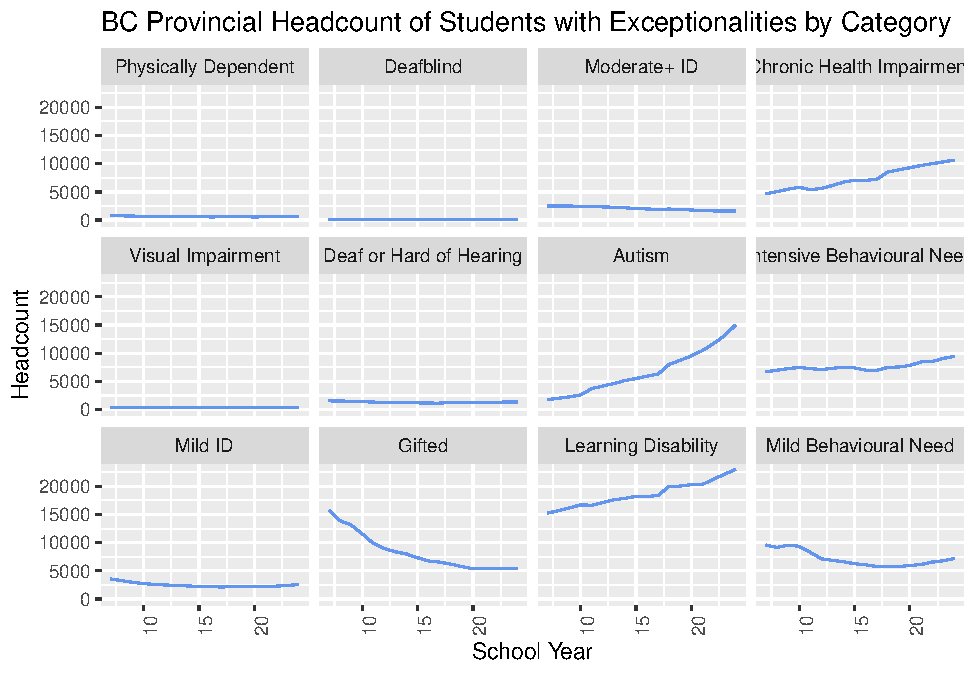
\includegraphics{draft_play_files/figure-latex/sandbox-1.pdf}

The district classification data was scaled down to include only public schools, while excluding private institutions. The school districts of Southeast Kootenay, Rocky Mountain, Kootenay Lake, Arrow Lakes, Revelstoke, Kootenay-Columbia, Cariboo-Chilcotin, Sea to Sky, Central Coast, Haida Gwaii, Boundary, Bulkley Valley, Nicola-Simikameen, Peace River South, Peace River North, Gulf Islands, Qualicum, Comox Valley, Campbell River, Gold Trail, Fraser-Cascade, Coast Mountains, Vancouver Island West, Vancouver Island North, Stikine, Nechako Lakes, Nisga'a, and Conseil scolaire francophone were excluded from the data set due to the lack of sufficient population information. The urban vs.~rural classifications were made based on the district's population on the 2016 census. If the population was above 100,000 individuals, it is classified as urban. If the population was below 99,999 individuals, then it is classified as rural.

This table displays the census results from 2011 and 2016 for our school districts. Many of the populations have stayed consistent within their urban or rural category. Three districts to note from the table are Nanaimo, Kamloops, and Chilliwack. In 2011, they were rural, but for our dataset they have been classified as urban due to their population increase in 2016.

\begin{verbatim}
## # A tibble: 198 x 18
##    year  disability    x6    x7    x8    x9   x10   x11   x12   x13   x14   x15
##    <chr> <chr>      <dbl> <dbl> <dbl> <dbl> <dbl> <dbl> <dbl> <dbl> <dbl> <dbl>
##  1 2002~ INTELLECT~   135   172   220   261   279   303   370   364   388   378
##  2 2002~ HEARING I~    46    66    69    67    79    78    69    70    53    72
##  3 2002~ SPEECH OR~  2502  2466  2443  2205  1894  1282   874   677   493   340
##  4 2002~ VISUAL IM~    18    27    25    16    12    26    19    24    31    19
##  5 2002~ EMOTIONAL~    81   178   241   292   347   433   504   487   549   548
##  6 2002~ ORTHOPEDI~    65    77    64    49    64    71    50    48    44    43
##  7 2002~ DEAF-BLIN~     0     2     0     0     1     0     2     0     4     2
##  8 2002~ MULTIPLE ~     0     0     0     0     0     0     0     0     0     0
##  9 2002~ AUTISM       267   289   290   334   325   316   290   256   243   219
## 10 2002~ TRAUMATIC~     6    11    17    23    22    19    21    23    36    36
## # ... with 188 more rows, and 6 more variables: x16 <dbl>, x17 <dbl>,
## #   x18 <dbl>, x19 <dbl>, x20 <dbl>, x21 <dbl>
\end{verbatim}

\begin{verbatim}
## # A tibble: 198 x 3
## # Groups:   year [18]
##     year disability                    total
##    <dbl> <chr>                         <dbl>
##  1  2002 AUTISM                         3339
##  2  2002 DEAF-BLINDNESS                   17
##  3  2002 DEVELOPMENTAL DELAY               0
##  4  2002 EMOTIONAL DISTURBANCE          4736
##  5  2002 HEARING IMPAIRMENT              873
##  6  2002 INTELLECTUAL DISABILITY        4387
##  7  2002 MULTIPLE DISABILITIES             0
##  8  2002 ORTHOPEDIC IMPAIRMENT           754
##  9  2002 SPEECH OR LANGUAGE IMPAIRMENT 15784
## 10  2002 TRAUMATIC BRAIN INJURY          306
## # ... with 188 more rows
\end{verbatim}

\begin{tabular}{r|l|r}
\hline
year & disability & total\\
\hline
2002 & AUTISM & 3339\\
\hline
2002 & DEAF-BLINDNESS & 17\\
\hline
2002 & DEVELOPMENTAL DELAY & 0\\
\hline
2002 & EMOTIONAL DISTURBANCE & 4736\\
\hline
2002 & HEARING IMPAIRMENT & 873\\
\hline
2002 & INTELLECTUAL DISABILITY & 4387\\
\hline
2002 & MULTIPLE DISABILITIES & 0\\
\hline
2002 & ORTHOPEDIC IMPAIRMENT & 754\\
\hline
2002 & SPEECH OR LANGUAGE IMPAIRMENT & 15784\\
\hline
2002 & TRAUMATIC BRAIN INJURY & 306\\
\hline
2002 & VISUAL IMPAIRMENT & 297\\
\hline
2003 & AUTISM & 3759\\
\hline
2003 & DEAF-BLINDNESS & 17\\
\hline
2003 & DEVELOPMENTAL DELAY & 0\\
\hline
2003 & EMOTIONAL DISTURBANCE & 4597\\
\hline
2003 & HEARING IMPAIRMENT & 811\\
\hline
2003 & INTELLECTUAL DISABILITY & 4351\\
\hline
2003 & MULTIPLE DISABILITIES & 0\\
\hline
2003 & ORTHOPEDIC IMPAIRMENT & 749\\
\hline
2003 & SPEECH OR LANGUAGE IMPAIRMENT & 15642\\
\hline
2003 & TRAUMATIC BRAIN INJURY & 300\\
\hline
2003 & VISUAL IMPAIRMENT & 295\\
\hline
2004 & AUTISM & 4341\\
\hline
2004 & DEAF-BLINDNESS & 12\\
\hline
2004 & DEVELOPMENTAL DELAY & 0\\
\hline
2004 & EMOTIONAL DISTURBANCE & 4661\\
\hline
2004 & HEARING IMPAIRMENT & 809\\
\hline
2004 & INTELLECTUAL DISABILITY & 4334\\
\hline
2004 & MULTIPLE DISABILITIES & 0\\
\hline
2004 & ORTHOPEDIC IMPAIRMENT & 741\\
\hline
2004 & SPEECH OR LANGUAGE IMPAIRMENT & 15627\\
\hline
2004 & TRAUMATIC BRAIN INJURY & 286\\
\hline
2004 & VISUAL IMPAIRMENT & 325\\
\hline
2005 & AUTISM & 4810\\
\hline
2005 & DEAF-BLINDNESS & 14\\
\hline
2005 & DEVELOPMENTAL DELAY & 0\\
\hline
2005 & EMOTIONAL DISTURBANCE & 4661\\
\hline
2005 & HEARING IMPAIRMENT & 799\\
\hline
2005 & INTELLECTUAL DISABILITY & 4218\\
\hline
2005 & MULTIPLE DISABILITIES & 0\\
\hline
2005 & ORTHOPEDIC IMPAIRMENT & 738\\
\hline
2005 & SPEECH OR LANGUAGE IMPAIRMENT & 15833\\
\hline
2005 & TRAUMATIC BRAIN INJURY & 273\\
\hline
2005 & VISUAL IMPAIRMENT & 301\\
\hline
2006 & AUTISM & 5459\\
\hline
2006 & DEAF-BLINDNESS & 12\\
\hline
2006 & DEVELOPMENTAL DELAY & 0\\
\hline
2006 & EMOTIONAL DISTURBANCE & 4662\\
\hline
2006 & HEARING IMPAIRMENT & 812\\
\hline
2006 & INTELLECTUAL DISABILITY & 4193\\
\hline
2006 & MULTIPLE DISABILITIES & 0\\
\hline
2006 & ORTHOPEDIC IMPAIRMENT & 742\\
\hline
2006 & SPEECH OR LANGUAGE IMPAIRMENT & 15956\\
\hline
2006 & TRAUMATIC BRAIN INJURY & 269\\
\hline
2006 & VISUAL IMPAIRMENT & 302\\
\hline
2007 & AUTISM & 6071\\
\hline
2007 & DEAF-BLINDNESS & 21\\
\hline
2007 & DEVELOPMENTAL DELAY & 0\\
\hline
2007 & EMOTIONAL DISTURBANCE & 4631\\
\hline
2007 & HEARING IMPAIRMENT & 835\\
\hline
2007 & INTELLECTUAL DISABILITY & 4121\\
\hline
2007 & MULTIPLE DISABILITIES & 0\\
\hline
2007 & ORTHOPEDIC IMPAIRMENT & 745\\
\hline
2007 & SPEECH OR LANGUAGE IMPAIRMENT & 16046\\
\hline
2007 & TRAUMATIC BRAIN INJURY & 258\\
\hline
2007 & VISUAL IMPAIRMENT & 325\\
\hline
2008 & AUTISM & 6571\\
\hline
2008 & DEAF-BLINDNESS & 15\\
\hline
2008 & DEVELOPMENTAL DELAY & 0\\
\hline
2008 & EMOTIONAL DISTURBANCE & 4671\\
\hline
2008 & HEARING IMPAIRMENT & 823\\
\hline
2008 & INTELLECTUAL DISABILITY & 4012\\
\hline
2008 & MULTIPLE DISABILITIES & 0\\
\hline
2008 & ORTHOPEDIC IMPAIRMENT & 746\\
\hline
2008 & SPEECH OR LANGUAGE IMPAIRMENT & 16116\\
\hline
2008 & TRAUMATIC BRAIN INJURY & 279\\
\hline
2008 & VISUAL IMPAIRMENT & 317\\
\hline
2009 & AUTISM & 7012\\
\hline
2009 & DEAF-BLINDNESS & 8\\
\hline
2009 & DEVELOPMENTAL DELAY & 0\\
\hline
2009 & EMOTIONAL DISTURBANCE & 4669\\
\hline
2009 & HEARING IMPAIRMENT & 830\\
\hline
2009 & INTELLECTUAL DISABILITY & 4000\\
\hline
2009 & MULTIPLE DISABILITIES & 0\\
\hline
2009 & ORTHOPEDIC IMPAIRMENT & 713\\
\hline
2009 & SPEECH OR LANGUAGE IMPAIRMENT & 16132\\
\hline
2009 & TRAUMATIC BRAIN INJURY & 283\\
\hline
2009 & VISUAL IMPAIRMENT & 314\\
\hline
2010 & AUTISM & 7357\\
\hline
2010 & DEAF-BLINDNESS & 8\\
\hline
2010 & DEVELOPMENTAL DELAY & -144\\
\hline
2010 & EMOTIONAL DISTURBANCE & 4638\\
\hline
2010 & HEARING IMPAIRMENT & 827\\
\hline
2010 & INTELLECTUAL DISABILITY & 3926\\
\hline
2010 & MULTIPLE DISABILITIES & -144\\
\hline
2010 & ORTHOPEDIC IMPAIRMENT & 718\\
\hline
2010 & SPEECH OR LANGUAGE IMPAIRMENT & 16354\\
\hline
2010 & TRAUMATIC BRAIN INJURY & 271\\
\hline
2010 & VISUAL IMPAIRMENT & 312\\
\hline
2011 & AUTISM & 7618\\
\hline
2011 & DEAF-BLINDNESS & 12\\
\hline
2011 & DEVELOPMENTAL DELAY & -36\\
\hline
2011 & EMOTIONAL DISTURBANCE & 4567\\
\hline
2011 & HEARING IMPAIRMENT & 810\\
\hline
2011 & INTELLECTUAL DISABILITY & 3830\\
\hline
2011 & MULTIPLE DISABILITIES & -144\\
\hline
2011 & ORTHOPEDIC IMPAIRMENT & 738\\
\hline
2011 & SPEECH OR LANGUAGE IMPAIRMENT & 16206\\
\hline
2011 & TRAUMATIC BRAIN INJURY & 268\\
\hline
2011 & VISUAL IMPAIRMENT & 313\\
\hline
2012 & AUTISM & 7888\\
\hline
2012 & DEAF-BLINDNESS & 10\\
\hline
2012 & DEVELOPMENTAL DELAY & -54\\
\hline
2012 & EMOTIONAL DISTURBANCE & 4524\\
\hline
2012 & HEARING IMPAIRMENT & 810\\
\hline
2012 & INTELLECTUAL DISABILITY & 3847\\
\hline
2012 & MULTIPLE DISABILITIES & -144\\
\hline
2012 & ORTHOPEDIC IMPAIRMENT & 705\\
\hline
2012 & SPEECH OR LANGUAGE IMPAIRMENT & 15938\\
\hline
2012 & TRAUMATIC BRAIN INJURY & 256\\
\hline
2012 & VISUAL IMPAIRMENT & 300\\
\hline
2013 & AUTISM & 8021\\
\hline
2013 & DEAF-BLINDNESS & 9\\
\hline
2013 & DEVELOPMENTAL DELAY & -36\\
\hline
2013 & EMOTIONAL DISTURBANCE & 4526\\
\hline
2013 & HEARING IMPAIRMENT & 830\\
\hline
2013 & INTELLECTUAL DISABILITY & 3847\\
\hline
2013 & MULTIPLE DISABILITIES & -144\\
\hline
2013 & ORTHOPEDIC IMPAIRMENT & 700\\
\hline
2013 & SPEECH OR LANGUAGE IMPAIRMENT & 16077\\
\hline
2013 & TRAUMATIC BRAIN INJURY & 254\\
\hline
2013 & VISUAL IMPAIRMENT & 288\\
\hline
2014 & AUTISM & 8364\\
\hline
2014 & DEAF-BLINDNESS & 5\\
\hline
2014 & DEVELOPMENTAL DELAY & -36\\
\hline
2014 & EMOTIONAL DISTURBANCE & 4577\\
\hline
2014 & HEARING IMPAIRMENT & 851\\
\hline
2014 & INTELLECTUAL DISABILITY & 3874\\
\hline
2014 & MULTIPLE DISABILITIES & -144\\
\hline
2014 & ORTHOPEDIC IMPAIRMENT & 673\\
\hline
2014 & SPEECH OR LANGUAGE IMPAIRMENT & 16236\\
\hline
2014 & TRAUMATIC BRAIN INJURY & 248\\
\hline
2014 & VISUAL IMPAIRMENT & 296\\
\hline
2015 & AUTISM & 8665\\
\hline
2015 & DEAF-BLINDNESS & 5\\
\hline
2015 & DEVELOPMENTAL DELAY & -36\\
\hline
2015 & EMOTIONAL DISTURBANCE & 4704\\
\hline
2015 & HEARING IMPAIRMENT & 844\\
\hline
2015 & INTELLECTUAL DISABILITY & 3951\\
\hline
2015 & MULTIPLE DISABILITIES & -144\\
\hline
2015 & ORTHOPEDIC IMPAIRMENT & 649\\
\hline
2015 & SPEECH OR LANGUAGE IMPAIRMENT & 16294\\
\hline
2015 & TRAUMATIC BRAIN INJURY & 240\\
\hline
2015 & VISUAL IMPAIRMENT & 291\\
\hline
2016 & AUTISM & 8940\\
\hline
2016 & DEAF-BLINDNESS & 8\\
\hline
2016 & DEVELOPMENTAL DELAY & 0\\
\hline
2016 & EMOTIONAL DISTURBANCE & 4944\\
\hline
2016 & HEARING IMPAIRMENT & 829\\
\hline
2016 & INTELLECTUAL DISABILITY & 4058\\
\hline
2016 & MULTIPLE DISABILITIES & -144\\
\hline
2016 & ORTHOPEDIC IMPAIRMENT & 624\\
\hline
2016 & SPEECH OR LANGUAGE IMPAIRMENT & 16075\\
\hline
2016 & TRAUMATIC BRAIN INJURY & 261\\
\hline
2016 & VISUAL IMPAIRMENT & 306\\
\hline
2017 & AUTISM & 9288\\
\hline
2017 & DEAF-BLINDNESS & 12\\
\hline
2017 & DEVELOPMENTAL DELAY & 0\\
\hline
2017 & EMOTIONAL DISTURBANCE & 5122\\
\hline
2017 & HEARING IMPAIRMENT & 841\\
\hline
2017 & INTELLECTUAL DISABILITY & 4103\\
\hline
2017 & MULTIPLE DISABILITIES & -144\\
\hline
2017 & ORTHOPEDIC IMPAIRMENT & 612\\
\hline
2017 & SPEECH OR LANGUAGE IMPAIRMENT & 16087\\
\hline
2017 & TRAUMATIC BRAIN INJURY & 282\\
\hline
2017 & VISUAL IMPAIRMENT & 282\\
\hline
2018 & AUTISM & 9752\\
\hline
2018 & DEAF-BLINDNESS & 11\\
\hline
2018 & DEVELOPMENTAL DELAY & -36\\
\hline
2018 & EMOTIONAL DISTURBANCE & 5286\\
\hline
2018 & HEARING IMPAIRMENT & 848\\
\hline
2018 & INTELLECTUAL DISABILITY & 4167\\
\hline
2018 & MULTIPLE DISABILITIES & -144\\
\hline
2018 & ORTHOPEDIC IMPAIRMENT & 602\\
\hline
2018 & SPEECH OR LANGUAGE IMPAIRMENT & 16357\\
\hline
2018 & TRAUMATIC BRAIN INJURY & 294\\
\hline
2018 & VISUAL IMPAIRMENT & 269\\
\hline
2019 & AUTISM & 10290\\
\hline
2019 & DEAF-BLINDNESS & 21\\
\hline
2019 & DEVELOPMENTAL DELAY & 266\\
\hline
2019 & EMOTIONAL DISTURBANCE & 5568\\
\hline
2019 & HEARING IMPAIRMENT & 870\\
\hline
2019 & INTELLECTUAL DISABILITY & 4199\\
\hline
2019 & MULTIPLE DISABILITIES & -144\\
\hline
2019 & ORTHOPEDIC IMPAIRMENT & 562\\
\hline
2019 & SPEECH OR LANGUAGE IMPAIRMENT & 16423\\
\hline
2019 & TRAUMATIC BRAIN INJURY & 327\\
\hline
2019 & VISUAL IMPAIRMENT & 282\\
\hline
\end{tabular}

\begin{verbatim}
## Warning: Removed 12 row(s) containing missing values (geom_path).
\end{verbatim}

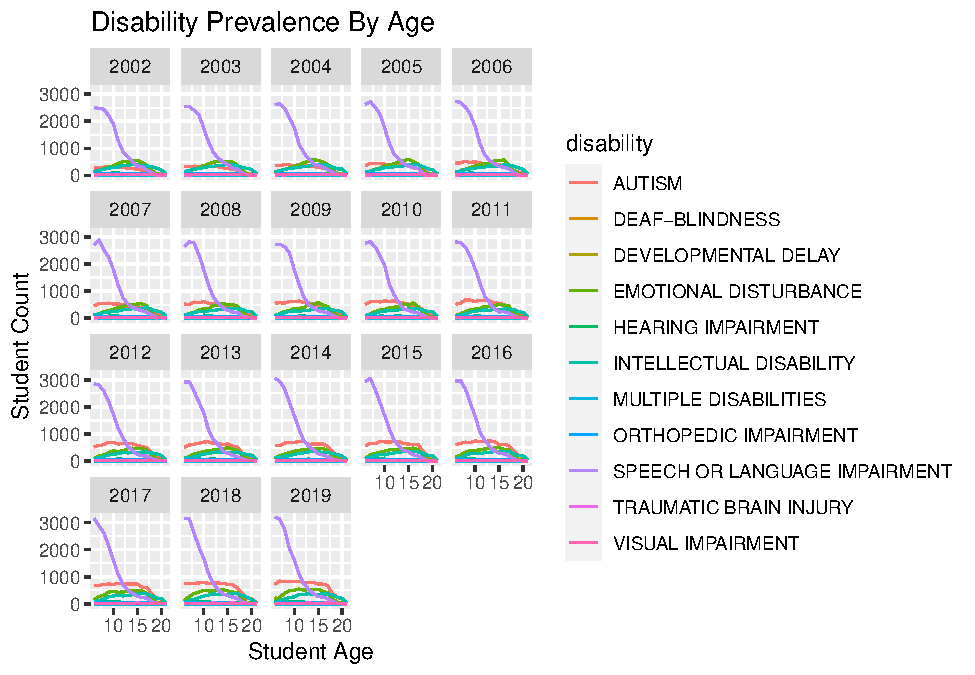
\includegraphics{draft_play_files/figure-latex/Oregon plot-1.pdf}

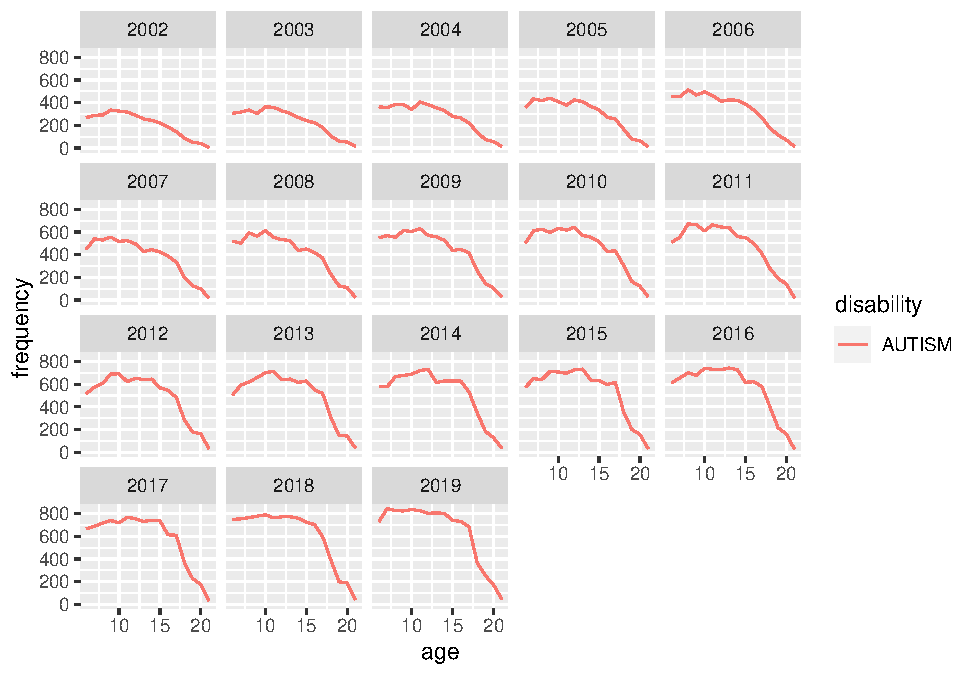
\includegraphics{draft_play_files/figure-latex/unnamed-chunk-2-1.pdf}

\begin{verbatim}
## Warning: Removed 190 rows containing non-finite values (stat_smooth).
\end{verbatim}

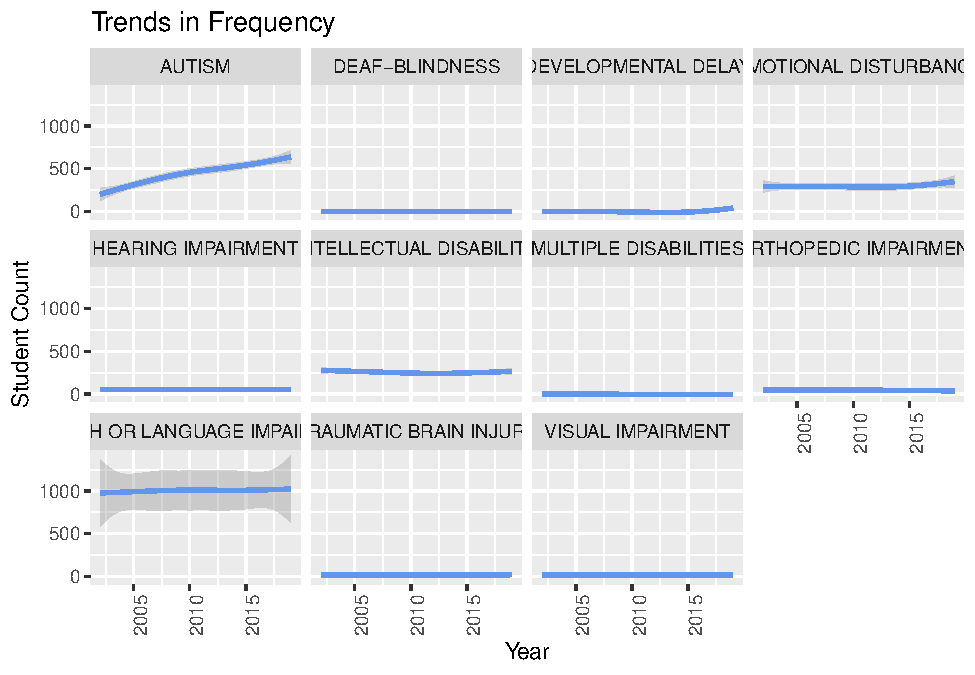
\includegraphics{draft_play_files/figure-latex/unnamed-chunk-3-1.pdf}

\hypertarget{procedure}{%
\subsection{Procedure}\label{procedure}}

\hypertarget{data-analysis}{%
\subsection{Data analysis}\label{data-analysis}}

We used R (Version 3.6.1; R Core Team, 2020) and the R-package \emph{papaja} (Version 0.1.0.9997; Aust \& Barth, 2020) for all our analyses.

\hypertarget{results-1}{%
\section{Results}\label{results-1}}

\hypertarget{discussion}{%
\section{Discussion}\label{discussion}}

\newpage

\hypertarget{references}{%
\section{References}\label{references}}

\begingroup
\setlength{\parindent}{-0.5in}
\setlength{\leftskip}{0.5in}

\hypertarget{refs}{}
\leavevmode\hypertarget{ref-R-papaja}{}%
Aust, F., \& Barth, M. (2020). \emph{papaja: Create APA manuscripts with R Markdown}. Retrieved from \url{https://github.com/crsh/papaja}

\leavevmode\hypertarget{ref-R-base}{}%
R Core Team. (2020). \emph{R: A language and environment for statistical computing}. Vienna, Austria: R Foundation for Statistical Computing. Retrieved from \url{https://www.R-project.org/}

\endgroup


\end{document}
